Until now, it has all been about preparing and installing Ubuntu on your system. This chapter is more like an orientation session where the various elements of the Ubuntu desktop are introduced to get you acquainted to using Ubuntu. Figure \ref{fig:ubuntu-desktop1} shows the default Ubuntu desktop. \\

\begin{figure}[h]	
	\centering
	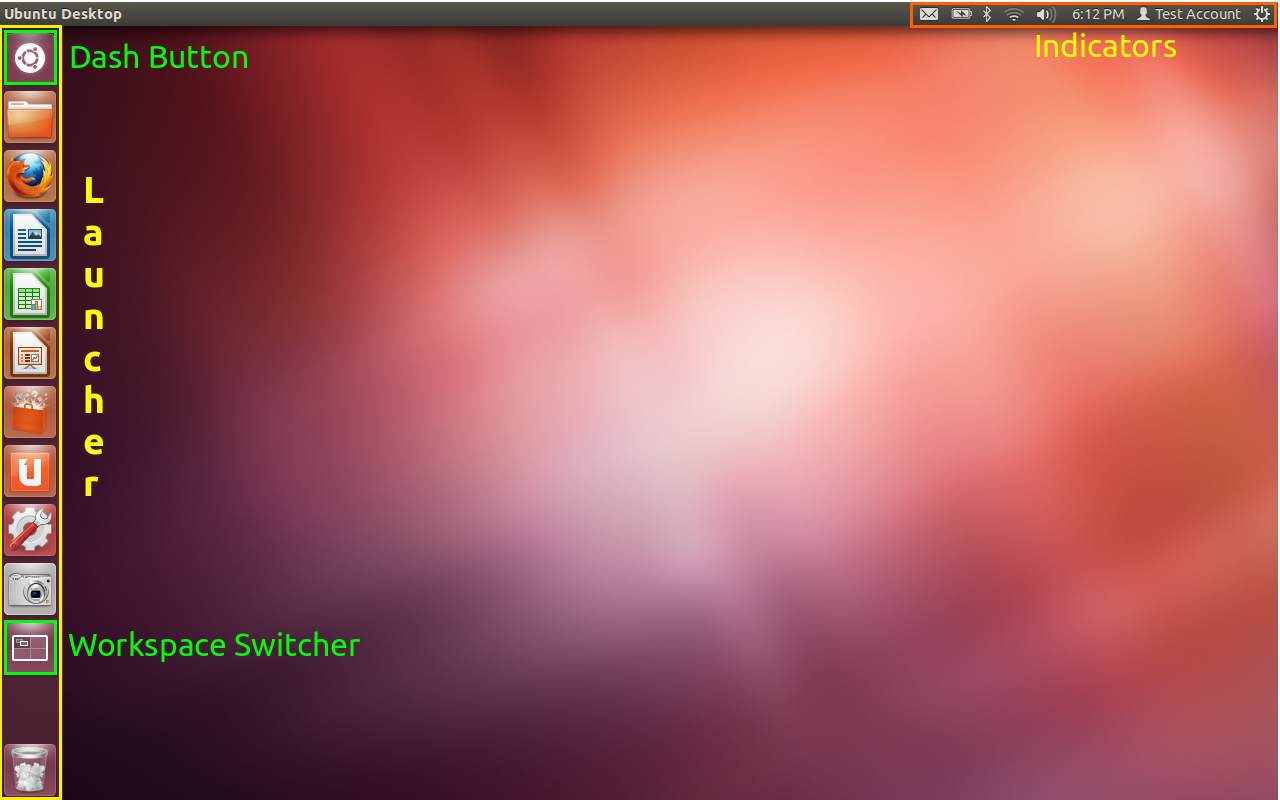
\includegraphics[width=400pt]{./images/desktop/desktop.png}
	\caption{Ubuntu Desktop}	
	\label{fig:ubuntu-desktop1}		
\end{figure}

\par \noindent Let's go through the various elements one by one starting with the launcher.  While describing the elements, it is also explained on how to use that element.

\section{Launcher} \index{Unity!Launcher}
The stack of icons on the left-hand side of the desktop (indicated by a yellow box) is called the Launcher. As the name suggests, its purpose is to help launch applications and performs the following functions.

\begin{itemize}
	\item Behave like a dock or start menu - You can pin your favourite applications for easy launch
	\item Shows the currently running applications
	\item Shows the status of the application (download progress, file copy progress etc)
	\item Shows external devices such as USB, external hard drive etc.
\end{itemize}

\par \noindent The launcher can be compared to the Windows Start panel or the Mac OS dock. You can launch an application by clicking on an application icon. If you want to remove the application  from the launcher, simply right-click the application icon and press ``Unlock from launcher".\\

\par \noindent The launcher also shows the currently running applications using small triangles. A white triangle is shown on the left side of an application icon to indicate that it is open. On the other hand, a white triangle is placed on the right side of the application if it is the currently focussed application. In figure \ref{fig:unity-applications}, the File manager and Firefox are open which is indicated by the white triangle on the left side of their icons. However, File manager is the application which is currently in focus, hence it also has a white triangle on the right side of its icon.

\begin{figure}[h]	
		\centering		
		\subfloat[State]
		{ 	\label{fig:unity-applications} 	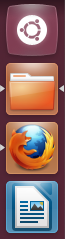
\includegraphics[width=40pt]{./images/desktop/applications.png} } 
		~ \hspace{1in}
		\subfloat[Move]
		{ 	\label{fig:unity-move-applications} 	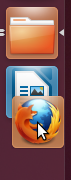
\includegraphics[width=50pt]{./images/desktop/move-applications.png}	}		
		\caption{Unity Launcher}
		\label{fig:unity-app}
\end{figure}

\par \noindent To indicate more than one instance of an application being open, two or three triangle depending on the number of instances appear on the left side of the icon. In figure \ref{fig:unity-move-applications}, there are two instances of the File manager open which is indicated by the two triangle to its left. You can also choose to rearrange applications in the launcher according to your preference. You can do this by pressing on the application icon, after a small delay the application slides out of its place as can be seen in \ref{fig:unity-move-applications}. You can now place it according to your preference. \\

\par \noindent The launcher can also be used to indicate the state, progress of an application. Basically the application icons indicate the progress of certain actions running in the background. This helps to keep track of the progress of an application action while actually working on something else. For instance, let's assume you are updating your system. You do not wait or keep checking the update manager to see if it is finished. You can meanwhile browse the web, check your email and keep an eye on the update manage application icon on the launcher. It shows the the number of updates and the update progress as seen in figure \ref{fig:update-number.png}. This is just one example. Several default applications in Ubuntu use this feature to display useful information using the launcher. Mozilla Thunderbird (default email client), Nautilus (default file manager) are few examples of such applications.\\

\begin{figure}[h]	
	\centering
	
\includegraphics[width=40pt]{./images/desktop/update-number.png}
	\caption{State, progress of the Update manager}	
	\label{fig:update-number.png}		
\end{figure}

\par \noindent Finally the launcher can also be used to open files quickly using a particular application quickly by simple drag and drop. For instance, if you wanted to open an image file, you can drag the image file to the launcher. The launcher will then automatically highlight only those applications which can open that file type. You have to then simply drop it on the application of your choice.

\section{Dash} \label{sect:dash} \index{Unity!Dash}
The Dash is a central place to search for applications, files, music, and videos, and show items you have used recently. It forms an important part of the Ubuntu desktop experience. No longer do you have to manually hunt for applications, files through the application menu or throught the folders etc. By default, you can search applications, files, folders, music and videos in the dash.  You can invoke the dash in figure \ref{fig:unity-dash}. You can show the dash by pressing the Super Key (Windows Key on most keyboards and the Cmd key on Apple keyboards) or by pressing the dash button as shown in figure \ref{fig:ubuntu-desktop1} indicated by the green box (ubuntu logo).\\

\begin{figure}[h]	
	\centering
	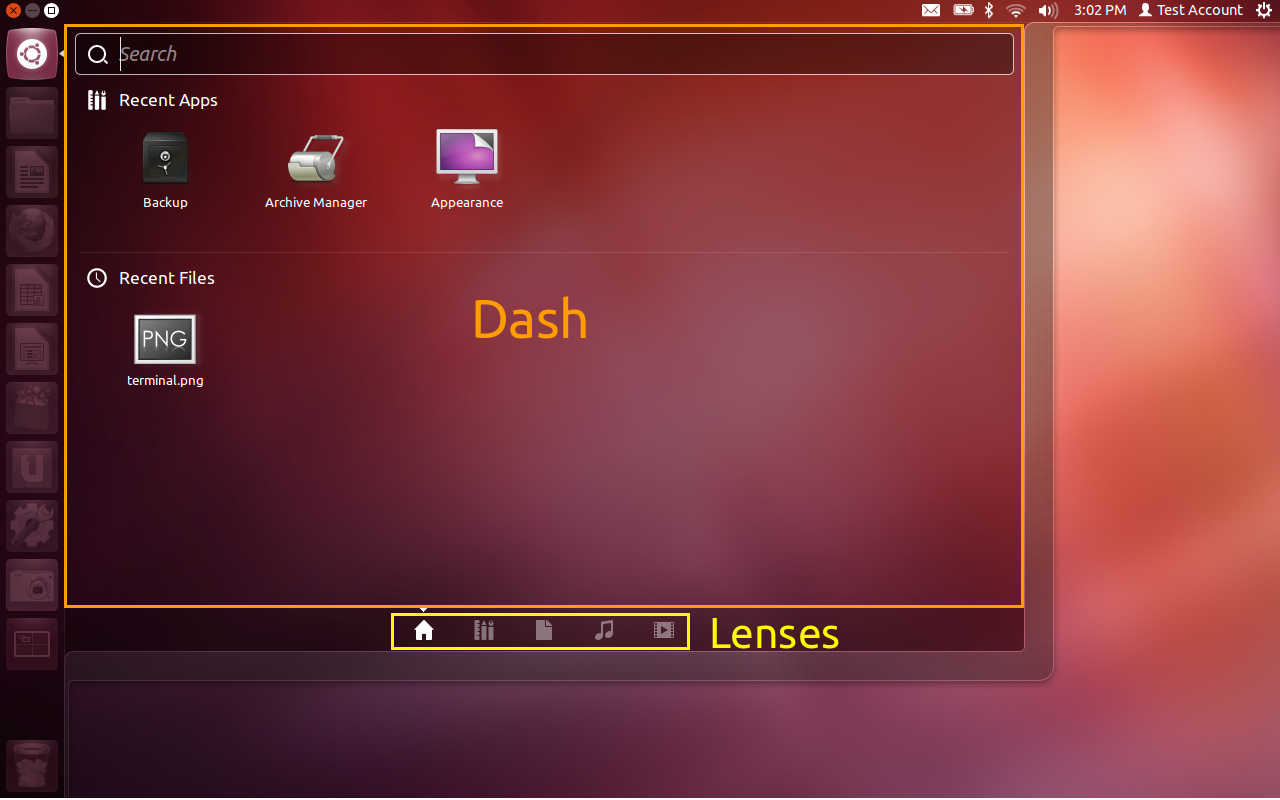
\includegraphics[width=400pt]{./images/desktop/dash.png}
	\caption{Unity Dash}	
	\label{fig:unity-dash}	
\end{figure}

\par \noindent The dash functionality can be extended to look for other stuff such as the web, youtube videos, cooking recipes directly from your dash by adding more lenses. Lenses \& Scopes are covered in more detail in the next section.  \\

\par \noindent Applications can now be quickly launched by pressing the Super key, type the application name and press enter to launch the application. \\

\par \noindent \framebox[6.7in][l]{\parbox[l]{6.5in}{\textbf{Tip}: You can pin any application to the launcher by dragging the application from the dash to the launcher and then right-clicking the application and pressing ``Lock to Launcher". If the application is already running, then you need to right click on the application icon in the launcher and then click on "Lock to launcher".}}

%\fbox{Tip: Quickly launch applications}

\section{Lenses \& Scopes} \index{Unity!Lenses}
Lenses are filters to show you only a specific type of data. You can see the lenses in figure \ref{fig:unity-dash} indicated by a yellow box. The lens In order of appearance (from the left to the right) are Home Lens, Application Lens, Files and Folders Lens, Music Lens and Video Lens. If you navigate to a specific lens like for instance the Music Lens, only your music files are shown while similarly only applications are shown in the Application lens. \\

\par \noindent Scopes are the back-end of lens as they dictate the sources where the information is gathered from. For instance, the file scope searches your hard disk for files and folder and displays it through the Files and Folders lens. It was mentioned before that the dash functionality could be extended. Well, this can be done by adding more lens which lets you search for other information as well. Additional lens can be installed from the Ubuntu Software Center. More about installing lens and applications are covered in chapter \ref{chap:software_management}. \\

\par \noindent \framebox[6.7in][l]{\parbox[l]{6.5in}{\textbf{Tip}: You can use the dash to quickly search for files and folder by using the file and folders lens.}}

\section{Top Panel and Indicators} \index{Indicators}
The top panel is the dark panel which can be seen in the top-hand of the desktop. At the top-right-hand side you can see some icons. This is illustrated by an orange box as can be seen in figure \ref{fig:ubuntu-desktop1}. The indicator as the name suggests are menus which indicate the status of applications. In order of appearance (from the left to the right) the indicators are messaging menu, battery menu, bluetooth menu, network menu, sound menu, clock, user menu and finally the system menu as can be seen in figure \ref{fig:unity-indicators}.

\begin{figure}[h]	
	\centering
	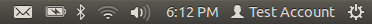
\includegraphics[width=200pt]{./images/desktop/indicators.png}
	\caption{Indicators}	
	\label{fig:unity-indicators}		
\end{figure}

\begin{description}
	\item [Messaging menu] Easily launch and receive incoming notifications from messaging applications including email, social networking, and Internet chat.	
	\item [Battery menu] Check your laptop battery's charging status. This menu is hidden by default if a battery isn't detected.	
	\item [Bluetooth menu] Send or receive files by Bluetooth. This menu is hidden by default if a supported Bluetooth device isn't detected.	
	\item [Network menu] Connect to wired, wireless, mobile, and VPN networks.	
	\item [Sound menu] Set the volume, configure sound settings, and control media players like Vlc, Spotify, Rhythmbox.	
	\item [Clock] Access the current time and date.	
	\item [User menu] Change your password, language settings or login picture. Quickly switch between user accounts without logging out.	
	\item [System menu] Access system settings. Lock screen, log out, suspend, restart or shutdown your computer.	
\end{description}

\par \noindent Applications like Spotify and Rhythmbox (default Ubuntu music player) integrate into the sound menu. They automatically run in the background when you close them. You can control them directly from the sound menu without having to actually open that application. This can be seen in figure \ref{fig:sound-menu}. 

\begin{figure}[h]	
		\centering		
		\subfloat[Sound Menu]
		{ 	\label{fig:sound-menu} 	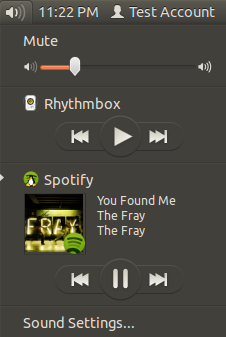
\includegraphics[width=100pt]{./images/desktop/sound-menu.png} } 
		~ \hspace{1in}
		\subfloat[Messaging Menu]
		{ 	\label{fig:messaging-menu} 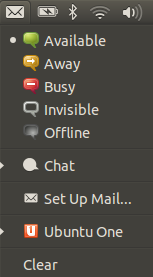
\includegraphics[width=90pt]{./images/desktop/messaging-menu.png}	}		
		\caption{Indicator Menus}
		\label{fig:unity-indicator-menus}
\end{figure}

\par \noindent Another useful indicator menu is the messaging menu. This menu is related to the social and communication related applications. Chat applications such as Empathy, Pidgin are integrated in this menu. This means that you can set the status of your messenger directly from this menu. It also provides option to set up your mail, and notifies you when new mail arrive. The messaging menu can be seen in figure \ref{fig:messaging-menu}.

\section{Heads Up Display - HUD} \label{sect:desktop-hud} \index{Heads Up Display}
%Definitely needs a screenshot in this section.
The Heads Up Display (HUD) is an intelligent search based approach to finding and accessing menu items you need. HUD automatically prioritises items that you frequently for easy access. How is this useful? Imagine you are using a new application. You no longer need to remember where a specific menu item is by hunting for it through the menus. With HUD, you can quickly search the task you want to perform and HUD will automatically show you the menu item you were looking for.  You can invoke the HUD by pressing the Alt key.\\

\begin{figure}[h]	
	\begin{center}
	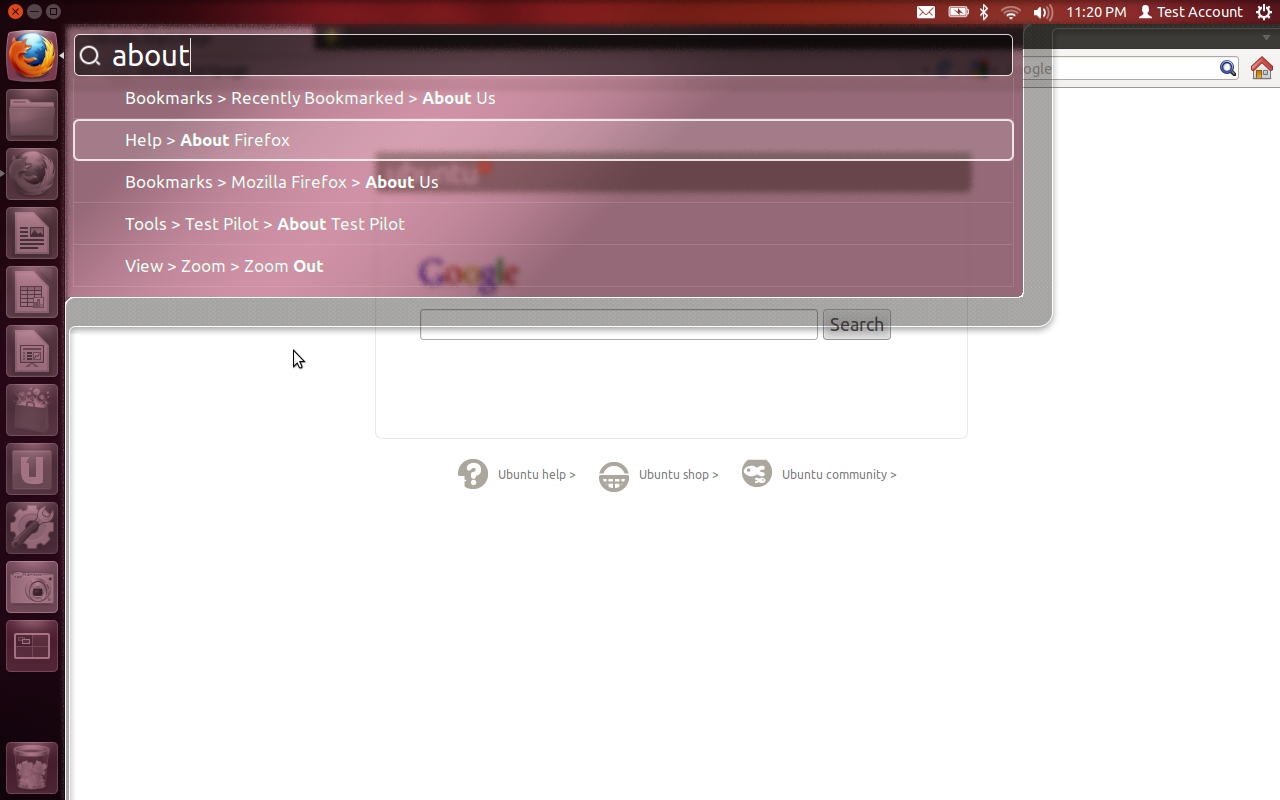
\includegraphics[width=400pt]{./images/desktop/HUD-firefox.png}
	\caption{Heads Up Display (HUD)}	
	\label{fig:unity-hud}	
	\end{center}
\end{figure}

\par \noindent For instance, let's assume a user using Firefox. If he want to customize his add-ons, he no longer needs to go through all the menus to find out where the add-ons menu item is present. He can using the HUD, search add-ons and HUD will present you with the menu item to customize add-ons. This is just one such instance, imagine how handy it woud be in applications with a lot of menus like Gimp or Blender.



